\documentclass[journal]{IEEEtran}

% --- packages -------------------------------------------------------------
\usepackage{amsmath,amssymb,amsfonts}
\usepackage{booktabs}
\usepackage{array}
\usepackage{multirow}
\usepackage{graphicx}
\usepackage{tikz}
\usetikzlibrary{positioning,fit,backgrounds,arrows.meta,calc}
\usepackage[hidelinks]{hyperref}
\usepackage{url}

\newcommand{\chance}{0.25}

\begin{document}

\title{A Leakage-Safe Benchmark for Multimodal Auditory Attention Decoding}

\author{Anonymous submission}

\maketitle

% ==========================================================================
\section{Benchmark}
\label{sec:benchmark}

% --------------------------------------------------------------------------
\subsection{Motivation and Scope}
\label{sec:bench-motivation}

A dataset is only as useful as the evidence that it contains the signal it
claims to. For an auditory attention decoding (AAD) corpus this is subtle: the
electroencephalographic (EEG) correlate of selective attention is real but faint,
and the richness that makes a multimodal corpus valuable---simultaneous EEG, eye
tracking, egocentric scene video, head inertial measurement (IMU), and spatialized
multi-speaker audio---also multiplies the ways a decoder can appear to work while
decoding something other than the listener's neural state.

This benchmark makes three contributions. First, a \emph{methodological} one that
is its organizing thesis: on this kind of corpus, \emph{content-disjoint splits are
necessary but not sufficient} for an admissible neural claim, and must be paired
with an \emph{EEG-shuffle null}. We show that a model with a learned stimulus
encoder can decode a stimulus-design confound (the attended talker is acoustically
marked) even on \emph{unseen} content, so no split removes it---only a null that
scrambles the EEG relative to the trial exposes whether a model's accuracy depends
on the brain at all. Second, we \emph{adjudicate} a public benchmark model under
this protocol and find its accuracy to be entirely non-neural, quantifying how much
of a headline number a split-only protocol can miss. Third, we provide a
\emph{truthful baseline}: an EEG-only stimulus-reconstruction decoder whose accuracy
is significantly above its own null, together with reference floors, the confound
characterization, and the decision-latency trade-off future methods should report.

We restrict the headline decoder to EEG, and report eye tracking, video, and IMU
only as \emph{characterization} branches (Section~\ref{sec:bench-results}); fusing
them is reserved for a companion method paper.

% --------------------------------------------------------------------------
\subsection{Task and Chance Level}
\label{sec:bench-task}

Each trial presents four attendable talkers from fixed loudspeakers (plus two
distractor loudspeakers that are never attended); the listener attends one and is
tested for comprehension. The benchmark task is the four-way identification of the
attended talker, evaluated as a \emph{match--mismatch} decision. From EEG we
reconstruct a feature $\hat{\mathbf r}\in\mathbb R^{d\times T}$ of the attended
speech and score each of the four real, co-present talker envelopes $\mathbf c_k$
by their correlation,
\begin{equation}
s_k=\frac{1}{d}\sum_{b=1}^{d}\tanh^{-1}\!\big(\rho(\hat{\mathbf r}_b,\tilde{\mathbf c}^{\,k}_b)\big),
\qquad \hat y=\arg\max_k s_k,
\label{eq:corr}
\end{equation}
where $\rho$ is the Pearson correlation over time, $\tilde{\mathbf c}$ is the
per-band $z$-scored candidate, and the Fisher $z$-transform is applied before the
band average. Because the four candidates are the four \emph{real} talkers present
in every window, the number of choices is exactly four at any window length; the
theoretical chance level is thus $\chance$ at every decision window, from $5$~s to
the whole $\approx\!30$~s trial. This is the property a four-way baseline must have,
and the reason we decode over the real co-present talkers rather than time-shifted
surrogates, whose chance level drifts with window length.

Two corpus confounds are defused \emph{architecturally}. \emph{Loudness:} the
attended talker is mixed to be attendable, but \eqref{eq:corr} is scale-free, so an
uninformative reconstruction correlates $\approx\!0$ with every candidate and
amplitude cannot help. \emph{Clip identity and the deterministic schedule:} the same
stimuli replay to every subject and the attended talker follows a fixed rotation, so
we \emph{permute} the four candidate streams per (subject,trial) and predict the
attended \emph{slot}; the same stimulus lands on different slots for different
subjects, and the decoder has no path from audio to the label except through the
EEG-derived reconstruction in \eqref{eq:corr}.

% ---- model figure --------------------------------------------------------
\begin{figure*}[t]
\centering
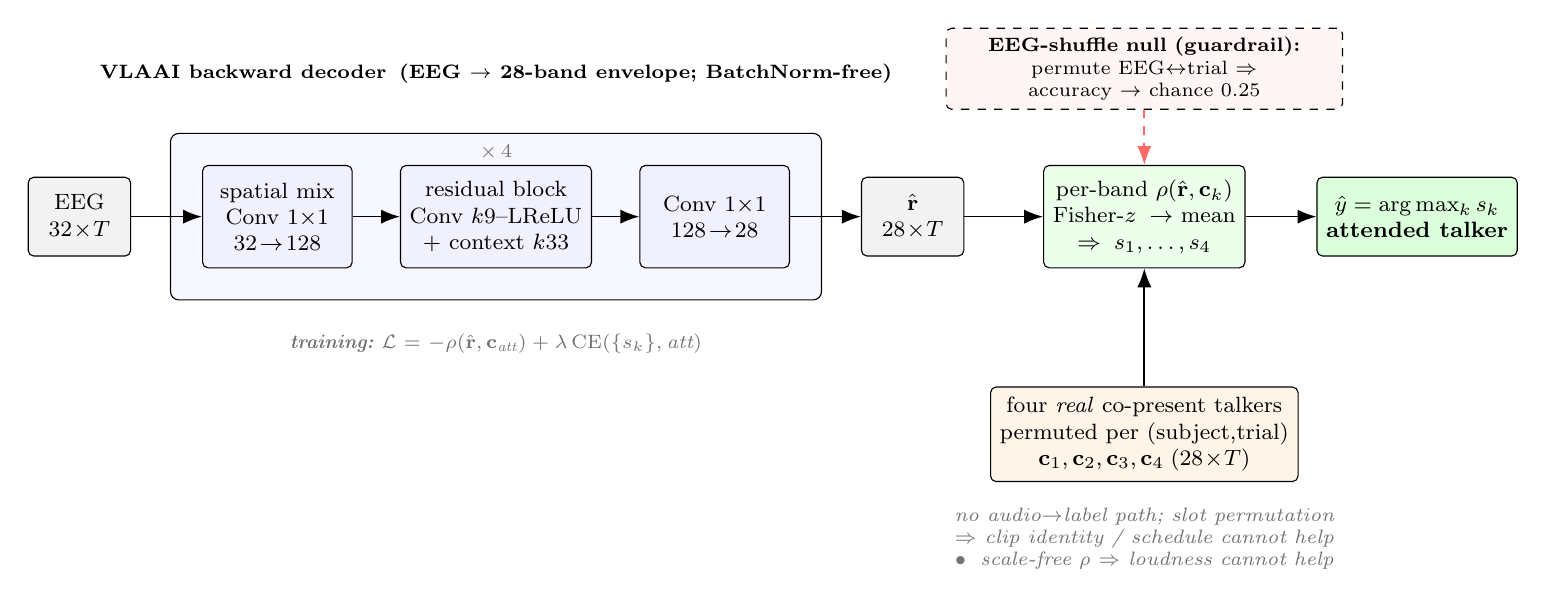
\begin{tikzpicture}[
  font=\footnotesize,
  io/.style={draw,rounded corners=2pt,align=center,minimum height=10mm,fill=black!5},
  blk/.style={draw,rounded corners=2pt,align=center,minimum height=13mm,minimum width=19mm,fill=blue!6},
  op/.style={draw,rounded corners=2pt,align=center,minimum height=13mm,fill=green!8},
  cnd/.style={draw,rounded corners=2pt,align=center,minimum height=12mm,fill=orange!9},
  note/.style={align=center,text=black!55,font=\scriptsize\itshape},
  fl/.style={-{Latex[length=2.4mm]},semithick},
]
\node[io,minimum width=13mm] (eeg) {EEG\\$32\!\times\!T$};
\node[blk,right=9mm of eeg] (b1) {spatial mix\\Conv $1{\times}1$\\$32\!\to\!128$};
\node[blk,right=6mm of b1] (b2) {residual block\\Conv $k9$--LReLU\\$+$ context $k33$};
\node[note] at ([yshift=1.6mm]b2.north) {$\times\,4$};
\node[blk,right=6mm of b2] (b3) {Conv $1{\times}1$\\$128\!\to\!28$};
\begin{scope}[on background layer]
  \node[draw,rounded corners=3pt,fit=(b1)(b2)(b3),inner sep=4mm,fill=blue!3] (dec){};
\end{scope}
\node[font=\scriptsize\bfseries,anchor=south] at ([yshift=5mm]dec.north)
  {VLAAI backward decoder\, (EEG $\to$ 28-band envelope; BatchNorm-free)};
\node[io,right=9mm of b3,minimum width=13mm] (rhat) {$\hat{\mathbf r}$\\$28\!\times\!T$};
\node[op,right=10mm of rhat,minimum width=24mm] (corr)
  {per-band $\rho(\hat{\mathbf r},\mathbf c_k)$\\Fisher-$z\;\to$ mean\\$\Rightarrow\; s_1,\dots,s_4$};
\node[io,right=9mm of corr,minimum width=17mm,fill=green!14] (yhat)
  {$\hat y=\arg\max_k s_k$\\\textbf{attended talker}};
\node[cnd,below=15mm of corr,minimum width=34mm] (cand)
  {four \emph{real} co-present talkers\\permuted per (subject,trial)\\$\mathbf c_1,\mathbf c_2,\mathbf c_3,\mathbf c_4\;(28\!\times\!T)$};
% main flow
\draw[fl] (eeg)--(b1);
\draw[fl] (b1)--(b2);
\draw[fl] (b2)--(b3);
\draw[fl] (b3)--(rhat);
\draw[fl] (rhat)--(corr);
\draw[fl] (corr)--(yhat);
\draw[fl] (cand.north)--(corr.south);
% training loss
\node[note,below=3mm of dec,text width=54mm]
  {\textbf{training:}\ $\mathcal L=-\rho(\hat{\mathbf r},\mathbf c_{\text{att}})+\lambda\,\mathrm{CE}(\{s_k\},\text{att})$};
% confound defusals
\node[note,below=2mm of cand,text width=60mm]
  {no audio$\to$label path; slot permutation $\Rightarrow$ clip identity / schedule cannot help
   \;$\bullet$\; scale-free $\rho$ $\Rightarrow$ loudness cannot help};
% null guardrail
\node[draw,dashed,rounded corners=2pt,fill=red!4,align=center,font=\scriptsize,
      text width=48mm,above=7mm of corr] (null)
  {\textbf{EEG-shuffle null (guardrail):}\\ permute EEG$\leftrightarrow$trial $\Rightarrow$ accuracy $\to$ chance $0.25$};
\draw[fl,dashed,red!60] (null.south)--(corr.north);
\end{tikzpicture}
\caption{\textbf{The benchmark decoder and its admissibility controls.} A VLAAI-style
backward network reconstructs the attended talker's $28$-band envelope $\hat{\mathbf r}$
from $32$-channel EEG---a $1{\times}1$ spatial mix, four residual convolutional blocks with
output-context temporal mixing, and a $1{\times}1$ projection, with no batch normalization.
The four \emph{real} co-present talker envelopes, permuted per (subject,trial), are scored by
their per-band Fisher-$z$ correlation with $\hat{\mathbf r}$ \eqref{eq:corr}; $\arg\max$ gives
the attended talker (chance $\chance$ at every window). The scale-free correlation defuses
loudness and the slot permutation defuses clip identity and the deterministic schedule; because
the decoder has \emph{no audio-to-label path}, the EEG-shuffle null---permuting the EEG against
the trial---drops accuracy to chance, certifying the decision is neural
(Section~\ref{sec:bench-admissibility}). A covert-spatial branch (gaze-residualized posterior
$\alpha/\beta$ power $\to$ shrinkage LDA) is fused out-of-fold within-subject; gaze, video, and
IMU are reported only as orienting-characterization branches.}
\label{fig:model}
\end{figure*}

% --------------------------------------------------------------------------
\subsection{Admissibility: Two Necessary Controls}
\label{sec:bench-admissibility}

We call a four-way result \emph{admissible} only if it passes both of the following.

\textbf{(C1) Content-disjoint splits.} Because the same stimuli are replayed to
every subject, holding out a subject does not hold out the audio. We therefore split
by trial content: a \texttt{trial\_k} in test appears in neither train nor
validation. \emph{within}-subject uses a per-subject $5$-fold over trial content;
\emph{leave-one-subject-out} (LOSO) holds out the subject \emph{and} the content
(test = the held-out subject's held-out trials; train/validation = the other fifteen
subjects' remaining content). Streams are read from a single pre-aligned
representation (per-stream recording lags resolved once, audio resampled to a common
$64$~Hz grid), so cross-modal misalignment cannot be reintroduced, and models are
BatchNorm-free so no train-subject statistic leaks under LOSO.

\textbf{(C2) EEG-shuffle null.} We permute the test EEG across trials so the brain
data no longer matches the trial's candidates (same EEG, candidates, and labels;
averaged over shuffles). A decoder that uses the EEG collapses to chance; a decoder
that ignores the EEG is unchanged. \emph{The null is a property of the model, not the
data:} two models on identical data can have very different nulls because the null
measures which input a model routes its decision through. A model is admissible only
if its accuracy is significantly above \emph{its own} null (paired one-sided $t$).

\textbf{Why C1 alone is insufficient.} The attended talker is systematically enhanced
by the stimulus design, leaving a \emph{general} acoustic marking present in every
trial, unseen ones included. A model with a learned \emph{audio} encoder can detect
this ``attended-style'' envelope on any track, so its accuracy survives
content-disjoint splitting---the confound is a stimulus-design property, not track
memorization, and no split can remove it. Only C2 reveals whether a given model
exploits it. A causal-lag control (accuracy at positive vs.\ negative EEG-to-audio
lag; genuine cortical tracking is causal, with audio leading EEG by
$\approx\!100$--$250$~ms) is logged as a secondary check.

% --------------------------------------------------------------------------
\subsection{Models}
\label{sec:bench-models}

\textbf{Content decoder (headline).} A \emph{backward} (stimulus-reconstruction)
network maps EEG to a speech feature and decides by \eqref{eq:corr} (Fig.~\ref{fig:model}).
The headline model is VLAAI-style \cite{accou2023vlaai}: a learned $32\!\to\!128$ spatial
projection, four residual convolutional blocks with output-context temporal mixing,
and a $1{\times}1$ projection to a $28$-band mel-spectrogram target; \emph{no}
batch normalization. Two confound-free additions are used: \emph{multi-band}
reconstruction (fuse per-band correlations via the Fisher $z$-transform of
\eqref{eq:corr}) and a \emph{match--mismatch margin} (an auxiliary cross-entropy
over the four candidate correlations). Accuracies are $5$-seed reconstruction
ensembles. A fully-convolutional decoder trained at $5$~s scores at any window, so
we report a \emph{decision-window curve}.

\textbf{Reference floor.} A single causal $\mathrm{Conv1d}$ integrating a
$\approx\!1$~s lag across channels---the classical linear AAD decoder
\cite{osullivan2015,wong2018,fuglsang2017}. It is the field-canonical floor and, as
shown below, sits at chance, certifying the task admits no trivial linear leak.

\textbf{Adjudicated prior.} We port the public benchmark's classifier
\cite{maestro}: dilated-convolutional encoders for EEG \emph{and} for each candidate
audio into a common space, with a learned cosine-similarity head and a softmax over
candidates. Its \emph{learned audio encoder} is precisely the ``audio-to-label
path'' that C2 is designed to expose.

\textbf{Covert-spatial branch.} Log $\alpha$/$\beta$ band-power over posterior
channels, \emph{gaze-residualized} (the window's gaze is regressed out with a
train-fold fit) and classified by a shrinkage LDA \cite{ledoit2004}; it reads covert
neural direction, not eye movements. It is fused with the content decoder by a late
weight tuned strictly out-of-fold.

\textbf{Overt-orienting characterization branches.} Two-dimensional gaze, frozen
scene+fovea video embeddings (a self-supervised encoder \cite{vjepa2}), and a head-IMU
summary, each decoded for attended \emph{direction} and attended \emph{content}.
These delimit the confounds and are not part of the headline decoder.

% --------------------------------------------------------------------------
\subsection{Training}
\label{sec:bench-training}

Content decoders reconstruct the attended feature under a negative-Pearson loss with
AdamW, cosine schedule with warmup, gradient clipping, and early stopping on
inner-validation match--mismatch accuracy; the VLAAI model uses learning rate
$10^{-3}$, weight decay $10^{-4}$, batch $128$, dropout $0.2$, up to $60$--$80$
epochs, and margin weight $0.3$. Each seed's reconstruction is $z$-scored over time
and averaged before \eqref{eq:corr}. Training windows are $5$~s with $50\%$ overlap;
the spatial LDA and overt classifiers are refit per evaluated window. The adjudicated
prior is trained with its published recipe (Adam, label smoothing, early stopping on
inner-validation) but under C1/C2.

% --------------------------------------------------------------------------
\subsection{Results}
\label{sec:bench-results}

Accuracies are means over $16$ subjects, held-out test, four-way (chance $\chance$);
``null'' is the EEG-shuffle null and ``margin'' is accuracy minus null.

\textbf{Admissibility, side by side.} Table~\ref{tab:adjud} reports the $5$~s point
under C1. Our decoder is significantly above its null in both protocols; the linear
decoder is at chance (no trivial leak); and the adjudicated prior's accuracy
\emph{equals its own null}---content-disjoint splitting does not lower it, because
its learned audio encoder reads the acoustic marking on unseen tracks. Its higher raw
number is therefore not a better read of the brain: none of it is neural.

\begin{table}[t]
\centering
\caption{Four-way accuracy at $5$~s under content-disjoint splits (C1), with the
EEG-shuffle null (C2). Margin significance is a paired one-sided $t$ ($n{=}16$).}
\label{tab:adjud}
\small
\begin{tabular}{@{}llccc@{}}
\toprule
Model & Protocol & 4-way & null & margin ($p$) \\
\midrule
\textbf{Ours} (VLAAI, mb$+$margin) & LOSO   & 0.34 & 0.26 & $+0.07$ ($2\!\times\!10^{-6}$) \\
\textbf{Ours}                       & within & 0.30 & 0.26 & $+0.045$ ($7\!\times\!10^{-5}$) \\
Linear (reference floor)            & both   & 0.25 & 0.25 & $\approx 0$ (n.s.) \\
Adjudicated prior \cite{maestro}    & LOSO   & 0.362 & 0.362 & $-0.00$ (n.s.) \\
Adjudicated prior                   & within & 0.253 & 0.253 & $-0.00$ (n.s.) \\
\bottomrule
\end{tabular}
\end{table}

\textbf{Headline: decision-window curve.} Accuracy integrates over time
(Table~\ref{tab:curve}). The four-way rate rises with the window while the null stays
flat at $\approx\!0.26$, so the neural margin grows and stays highly significant; LOSO
reaches $0.497$ at the whole trial (margin $+0.23$, $p\!<\!10^{-13}$) and crosses
$0.40$ by $\approx\!15$~s.

\begin{table}[t]
\centering
\caption{Decision-window curve ($16$ subjects, VLAAI mb$+$margin). $\Delta$ is the
paired margin over the EEG-shuffle null; all $\Delta$ significant at $p<10^{-10}$.}
\label{tab:curve}
\small
\begin{tabular}{@{}lccc@{\hskip 10pt}ccc@{}}
\toprule
& \multicolumn{3}{c}{LOSO} & \multicolumn{3}{c}{within} \\
\cmidrule(lr){2-4}\cmidrule(lr){5-7}
Window & 4-way & null & $\Delta$ & 4-way & null & $\Delta$ \\
\midrule
$5$~s  & 0.348 & 0.266 & $+0.083$ & 0.317 & 0.259 & $+0.058$ \\
$10$~s & 0.383 & 0.264 & $+0.119$ & 0.336 & 0.261 & $+0.075$ \\
$15$~s & 0.431 & 0.264 & $+0.167$ & 0.354 & 0.257 & $+0.097$ \\
$20$~s & 0.440 & 0.262 & $+0.178$ & 0.343 & 0.256 & $+0.087$ \\
$30$~s & \textbf{0.497} & 0.267 & $+0.230$ & \textbf{0.406} & 0.261 & $+0.145$ \\
\bottomrule
\end{tabular}
\end{table}

\textbf{What raises the margin, and what does not.} We swept improvement levers under
C1/C2. The dominant lever is the decision window above. \emph{Multi-band $+$ margin}
adds a small significant gain over a plain envelope decoder (LOSO four-way $+0.020$,
$p{=}0.001$). \emph{K-shot subject calibration}---fine-tuning the LOSO model on $K$
of the held-out subject's own trials, disjoint from its test trials---adds
$+0.015$ margin at $K{=}20$ ($p{=}0.03$), saturating there. Two intuitive levers did
\emph{not} survive $16$-subject validation: an onset/edge (rectified-derivative)
target (within $\Delta$margin $-0.026$) and distractor hard-negatives (speakers
$5$--$6$). Throughout, the null remained at $0.25$--$0.26$: envelope-feature
engineering has plateaued, but every reported number is genuinely neural.

\textbf{Covert-spatial fusion} improves the within-subject four-way at every window
(e.g.\ $0.313\!\to\!0.347$ at $5$~s) because the cue is individually calibrated; under
LOSO the admissible cross-subject fusion weight goes to zero at every window---the
covert-spatial cue is real per subject but does not transfer---so LOSO is carried by
content alone. Covert spatial fusion is thus a within-subject lever.

\textbf{Overt-orienting characterization.} Table~\ref{tab:overt} decodes direction and
content from the three non-EEG modalities. Each decodes \emph{direction} well above
chance and rising with the window; \emph{none} decodes \emph{content} above chance.
Vision is the strongest overt cue, the head IMU the weakest (no magnetometer, so head
yaw is only partly recoverable). The unanimity---orienting everywhere, content
nowhere---is why the spatial branch is gaze-residualized and the content task
permuted.

\begin{table}[t]
\centering
\caption{Overt-orienting reference branches: attended direction and content
(whole-trial four-way, chance $\chance$). ``$\approx$ch'' $=$ at chance at every window.}
\label{tab:overt}
\small
\begin{tabular}{@{}lcccc@{}}
\toprule
& \multicolumn{2}{c}{Direction} & \multicolumn{2}{c}{Content}\\
\cmidrule(lr){2-3}\cmidrule(lr){4-5}
Modality & within & LOSO & within & LOSO \\
\midrule
Gaze (2-D)            & 0.49--0.57 & 0.42--0.47 & $\approx$ch & $\approx$ch \\
Scene video           & 0.62--0.68 & 0.55--0.59 & $\approx$ch & $\approx$ch \\
Head IMU (accel+gyro) & 0.38--0.46 & 0.31--0.40 & $\approx$ch & $\approx$ch \\
\bottomrule
\end{tabular}
\end{table}

\textbf{The null level.} Theoretical chance is $\chance$ and a white-noise
reconstruction scores $0.250$ empirically, confirming the four candidates are a fair
choice. Our trained decoder's null instead sits, flatly, at $\approx\!0.265$: the
$0.015$ excess is the \emph{audio-only floor}---a decoder trained to reconstruct
attended envelopes matches the attended talker's marking slightly even with its EEG
scrambled. This offset is constant across windows, present equally in the real
accuracy, and removed by measuring the margin against the empirical null rather than
$\chance$; reporting against $\chance$ would overstate the effect.

% --------------------------------------------------------------------------
\subsection{Discussion}
\label{sec:bench-discussion}

\textbf{The central lesson.} Strict splits are not enough. A subject- and
content-disjoint protocol is standard practice, yet a model with a learned stimulus
encoder converted it back into an inadmissible result by reading the stimulus design
itself (Table~\ref{tab:adjud}): its accuracy is its own null. The EEG-shuffle null is
the control that catches this, and it is inexpensive---for a window-wise decoder it is
exactly a permutation of the reconstruction against the candidates. We recommend it as
a required control for any AAD leaderboard, alongside content-disjoint splits and a
reported chance level that is the \emph{empirical} null, not $1/K$.

\textbf{What the benchmark establishes.} The corpus carries genuine, confound-free
cortical attention signal: under C1/C2 the deep decoder is well above its null (LOSO
whole-trial $0.497$ vs.\ $0.267$, $p<10^{-13}$) while the linear floor is at chance.
The negative controls are as informative as the positive result---the linear floor
rules out a trivial leak, and the overt-modality branches (Table~\ref{tab:overt}) show
every strong non-neural cue is spatial, not content, so it cannot masquerade as talker
decoding once the task is permuted.

\textbf{Applicability.} The decision-window curve quantifies the accuracy--latency
trade-off any real-time selection system must navigate \cite{geirnaert2021}: usefully
above chance by $5$~s, approaching one-in-two at the whole trial. The within-vs-LOSO
gap and the $K$-shot curve quantify the calibration burden: a subject-independent model
is carried by content alone, while $\approx\!20$ calibration trials of a new user add a
small further gain and a subject-specific model can also exploit the covert-spatial
cue. The characterization branches tell a designer what each sensor buys---strong,
cheap orienting from gaze and video---and warn that none substitutes for the neural
content read-out.

\textbf{Limitations.} Envelope tracking here is genuinely weak, so absolute accuracies
are modest and envelope-feature engineering has plateaued (onset targets and
hard-negatives did not help). With $100$ trials per subject the whole-trial estimates
are noisy. The empirical null is $0.265$ rather than exactly $\chance$; we report
margins over it. The covert-spatial cue does not transfer across subjects, bounding a
subject-independent fusion.

\textbf{Headroom.} By construction the benchmark leaves room above it: the decoder is a
single reconstruction with a fixed correlation read-out. A learned similarity head
(added to our correlation front-end it is margin-neutral but---unlike the adjudicated
prior's audio encoder---keeps the null at $\approx\!0.26$, since it operates on
EEG-to-audio correlations rather than raw audio), reliability-weighted multimodal late
fusion, subject adaptation, and self-supervised pretraining are all untouched and are
the subject of the companion method paper. The benchmark's role is to fix the task,
the two admissibility controls, the windows, and the confound characterization on which
those methods should be judged.

% --- references -----------------------------------------------------------
\begin{thebibliography}{1}
\small
\bibitem{osullivan2015}
J.~A. O'Sullivan \emph{et al.}, ``Attentional selection in a cocktail party
environment can be decoded from single-trial EEG,'' \emph{Cereb.\ Cortex},
vol.~25, no.~7, pp.~1697--1706, 2015.

\bibitem{wong2018}
D.~D.~E. Wong \emph{et al.}, ``A comparison of regularization methods in forward and
backward models for auditory attention decoding,'' \emph{Front.\ Neurosci.}, vol.~12,
art.~531, 2018.

\bibitem{fuglsang2017}
S.~A. Fuglsang, T.~Dau, and J.~Hjortkj{\ae}r, ``Noise-robust cortical tracking of
attended speech in real-world acoustic scenes,'' \emph{NeuroImage}, vol.~156,
pp.~435--444, 2017.

\bibitem{accou2023vlaai}
B.~Accou, J.~Vanthornhout, H.~Van hamme, and T.~Francart, ``Decoding of the speech
envelope from EEG using the VLAAI deep neural network,'' \emph{Sci.\ Rep.}, vol.~13,
art.~812, 2023.

\bibitem{maestro}
ASPIRE-OSU, ``MAESTRO: a multimodal AAD benchmark,'' public code release, 2024.

\bibitem{geirnaert2021}
S.~Geirnaert \emph{et al.}, ``Electroencephalography-based auditory attention decoding:
Toward neurosteered hearing devices,'' \emph{IEEE Signal Process.\ Mag.}, vol.~38,
no.~4, pp.~89--102, 2021.

\bibitem{ledoit2004}
O.~Ledoit and M.~Wolf, ``A well-conditioned estimator for large-dimensional covariance
matrices,'' \emph{J.\ Multivariate Anal.}, vol.~88, no.~2, pp.~365--411, 2004.

\bibitem{vjepa2}
M.~Assran \emph{et al.}, ``V-JEPA~2: Self-supervised video representations,''
\emph{arXiv preprint}, 2025.
\end{thebibliography}

\end{document}
